\subsection{Convolutional Neural Networks}
\label{sec:neural-networks-convolutional-neural-networks}
Convolutional neural networks are suited for image processing tasks because they are invariant regarding the position of an object within an image.
Moreover, they need fewer parameters than multilayer perceptrons for finding features because the weights of local features can be shared and applied to different regions of an image \cite{LeCun1998cnn, Lecun98}.
Hence, they yield higher accuracies on generalized images in less training time.
The latter refers to the process of finding well-suited parameters.
Convolutional neural networks do not have an as strict separation in multiple layers as multilayer perceptrons do.
They rather have a pool of several layers which can be arbitrarily connected, repeated, and tuned with respect to their parameters to fulfill one's needs as illustrated in \figref{fig:cnn-layers}.
\begin{figure}
	\centering
	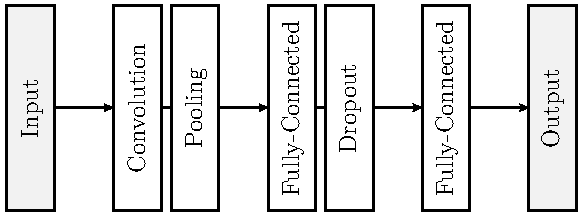
\includegraphics[]{images/cnn_layers.pdf}
	\caption[Layers of a convolutional neural network]{Layers of a convolutional neural network. Each combination of convolutional layer and pooling layer or fully-connected and dropout can be arbitrarily repeated. Moreover, pooling layers and dropout regularization layers are optional. The last fully-connected layer is not combined with a dropout layer.}
	\label{fig:cnn-layers}
\end{figure}
Commonly, convolutional layers are combined with pooling layers and fully-connected layers with dropout regularization layers.
However, the latter combinations are optional.
Each of them is explained in the following sections.
Combinations and repetitions of those layers with their own hyperparameters are called architecture.
Usually, convolutional and pooling layers manipulate the input and the resulting activations before fully-connected layers appear.
There are different proposed architectures with their weights and biases available.
The most common ones are AlexNet \cite{Krizhevsky:2012:ICD:2999134.2999257}, VGG \cite{Simonyan15}, GoogLeNet \cite{szegedy2015} and, ResNet \cite{He2016ResNet}.

\subsubsection{Convolutional Layer}
\label{sec:cnn-convolutional-layer}
The most important layer is the convolutional layer.
As the name suggests it performs a convolution with a filter matrix of arbitrary size on an input matrix of arbitrary size.
Let's say the input matrix is an image $\vec{X} \in \mathbb{R}^{m \times n}$.
The filter matrix $\vec{K} \in \mathbb{R}^{i \times j}$ contains $i \cdot j$ weights of the network.
The filter is now slid across the image and performs a dot product within its window.
\figref{fig:convolution} illustrates the following operation.
In reference to the figure the kernel covers the four elements in the top right corner of the input image.
Hence, the dot product multiplication for this setup yields $5 \cdot 1+4 \cdot -1+1 \cdot -1+3 \cdot 1=3$.
This result is stored in a new matrix at its corresponding place.
At the end, this matrix will hold all values of the convolution operation.
After each calculation of the dot product, the filter matrix moves.
The corresponding step size is called stride.
A stride of 1 moves the filter one pixel or element, respectively.
There can be a different stride along the $x$-axis and $y$-axis.
When the filter has moved across the whole input, the resulting matrix is completely filled up like the one in the figure.
This resulting matrix is called a feature map, because the convolution extracted features from its input.
\begin{figure}
	\centering
	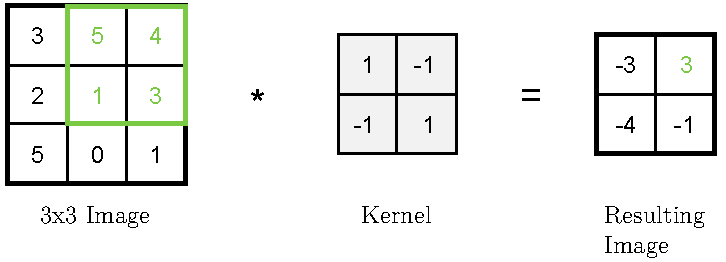
\includegraphics{images/convolution.pdf}
	\caption[Convolution of an Image with a Kernel]{Convolution of an image and a kernel. The $2 \times 2$ kernel is sled across the $3 \times 3$ image and performs a dot product multiplication within its window each time. Here, the kernel moves with a stride of 1, which results in the shown image on the right, the so called feature map.}
	\label{fig:convolution}
\end{figure}
Doing this operation the feature map is always smaller than the input.
Sometimes this is not desirable, because this means a loss in information.
If multiple convolutions are performed, the feature map constantly shrinks until no feature can be extracted anymore or only rough ones.
Thus, a padding $p$ can be applied to the input.
This means surrounding the input with $p$ rounds of zeros like it is illustrated in \figref{fig:convolution-padding} with $p=1$.
The convolution operates like usual, just on a larger input.
\begin{figure}
	\centering
	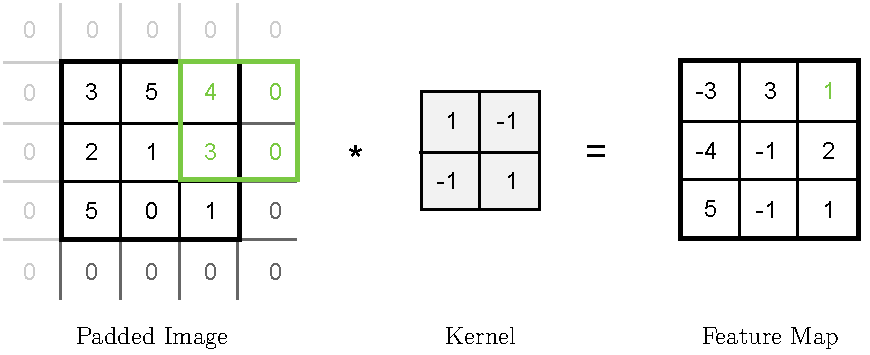
\includegraphics{images/convolution_padding.pdf}
	\caption[Convolution of a Padded Image with a Kernel]{Convolution of a padded image with a $2 \times 2$ kernel. The $3 \times 3$ image is surrounded with zeros for inducing its size to the feature map. However, the convolution operates like usual, just on a larger input. If the amount padding is odd, a padding at the right and at the bottom is preferred.}
	\label{fig:convolution-padding}
\end{figure}
In practical terms, there are two common conventions for convolutions: valid and same.
The former defines that no padding is applied and therefore a kind of valid convolution is performed, because only the real input is minded.
This means that the feature map has a size of $\vec{F} \in \mathbb{R}^{m-i+1 \times n-j+1}$.
The latter means, that the size of the feature map equals the one of the input.
How much padding $p$ needs to be applied can be calculated by comparing each matrix shapes and using
\begin{align}
	m &= m+2p-i+1 \\
	p &= \frac{i-1}{2}
\end{align}
as a general equation.
However, this only covers the padding height.
If the image or filter are not symmetrical, the padding along the width needs to be calculated as well by replacing $m$ with $n$ and $i$ with $j$.
Another remark is, that in computer vision filter sizes usually are odd.
There can be two reasons for this.
First, the filter has a center which helps to tell where exactly the filter points to.
Second, the padding $p$ is even.
Otherwise, it needs to be rounded up for a correct mathematical representation, but only used on two sides of the image like it is shown in the figure with the help of transparency.
Only the padding at the right and at the bottom are taken into account for creating a filter matrix with the same shape of the original input.

The kernel in the figure would find top-left to bottom-right diagonal lines, because those are the pixels weighted most.
Like this but with slightly larger kernels and different weights more complex features can be found.
It is also possible to perform multiple different convolutions on the same input for finding different features.
They are stored as a matrix, where every feature represents the depth of the feature map.
This whole process solves the limitation to a fixed position of features of the multilayer perceptrons architecture.
Even if, for example, a digit covers only have the image, all features are found, because the kernel is moved over the image and not single neurons or filters are responsible for single pixels.
Furthermore, because features are found by a moving filter, convolutional neural networks need way less weights and biases due to the possibility of reusing them.
The accuracy compared to multilayer perceptron networks is improved by concatenating several convolutions.
That means a convolution is performed on the feature map of an earlier convolution.
First, rough features like edges are found, and the deeper it gets into the network, the finer the features get.
\subsubsection{Pooling Layer}
\label{sec:cnn-pooling-layer}
After obtaining features using a convolutional layer a pooling layer can be inserted working on their activations.
Pooling serves as a spatial dimension reduction.
This is done by moving a filter $\vec{K} \in \mathbb{R}^{i \times j}$ with a given stride $s$ over an input $\vec{I} \in \mathbb{R}^{u \times v}$ that compresses the information or values, respectively, within its window.
However, the depth is usually not compressed and stays the same.
The objective of this process is to remove unnecessary information while keeping important features and improving computational power as less spatial information is available.
Hence, fewer weights and biases are needed which in turn improves training time.
\figref{fig:pooling} illustrates the pooling process for a max pooling operation in practical terms.
A max pooling filter $\vec{K}_{\text{max}}$ yields the maximum within its window as the result.
Moving such a $2 \times 2$ filter over an $4 \times 4$ input $\vec{I}$ with a stride of $s=2$ yields a matrix with each maximum at its corresponding position.
The maximum of the red colored $2 \times 2$ window is 7, hence, this number comes up in the result.
The other windows are processed identically.
The size of the result of an arbitrary pooling operation can be calculated with \eqref{eq:feature-map-shape} and $\dim \left( \vec{F} \right)_3 = \dim \left( \vec{I} \right)_3$.
Another pooling type is mean pooling.
Hereby, the result of each window is the mean of all its values.
In many architectures max pooling outperforms mean pooling \cite{Scherer2010}, however, in general, the type of pooling is problem-specific.
As it can be seen, pooling layers do not have learnable parameters only hyperparameters.
\begin{figure}
	\centering
	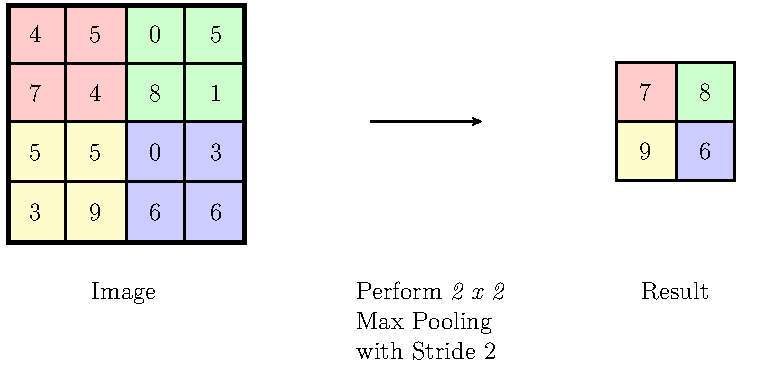
\includegraphics{images/pooling.pdf}
	\caption[Max pooling with $2 \times 2$ filter and stride $2$]{Max pooling with $2 \times 2$ filter $\vec{K}_{\text{max}}$ across a $4 \times 4$ input $\vec{I}$ with a stride of $s=2$. Within each window, the maximum of its values is computed. Finally, this yields a matrix with each maximum at its corresponding position.}
	\label{fig:pooling}
\end{figure}
\subsubsection{Fully-Connected Layer}
\label{sec:cnn-fully-connected}
The last part of a convolutional neural network mostly consists of at least one fully connected layer.
Such a layer is identical to a perceptron layer in \figref{fig:multilayer-perceptron} but uses the outputs or activations, respectively, of the previous convolutional or pooling layer.
The objective is to combine several features that were detected and use them as attributes for classifying the input.
Due to the weights, some attributes are more significant than others.
For example, if four legs and a long snout are found, there is a dog in the image and not a cat.
If the task is to distinguish only between cats and dogs, the snout feature is weighted more than the leg feature.
For preventing overfitting and improving generalization, a fully-connected layer can be combined with the dropout regularization technique \cite{Srivastava:2014:DSW:2627435.2670313}.
This drops out nodes randomly during training with a given probability, i.\,e. changing their incoming and outgoing weights temporarily to zero.
Hence, their weights are not adapted.
The interpretation of the activations of the last fully-connected layer in the architecture is simplified by applying an additional softmax function that squashes them into a range of 0 and 1, whereas the sum of all equals 1, to represent percentages of confidence or a probability distribution, respectively \cite{Bishop2006}.
The prediction $\hat{y}$ of a class $c$ manipulated with the softmax function can be written as
\begin{equation}
	\label{eq:softmax}
	\hat{y}_c = \frac{\exp(a^{[L]}_c)}{\sum_{j}^{n_y} \exp(a^{[L]}_j)}
\end{equation}
where $\vec{a}^{[L]}$ are the activations of the last layer.
Because the softmax manipulation outputs a probability distribution, it can only be performed when the classes are mutually exclusive, i.\,e. when only one class is correct.
Otherwise, for multi-label classification, a sigmoid function can be used, that squashes each output of the network into a range of 0 and 1.
The softmax or sigmoid manipulation corresponds to the output block in \figref{fig:cnn-layers}.
Combining the last fully-connected layer with a dropout layer is not desirable because this would remove some predictions of classes.